
\begin{exercise}\label{exercise-1_3-table1}
Use the numerically given function $f(x)$ below to find each of the following.

\begin{center}
\begin{tabular}{|c|c|c|c|c|c|c|} \hline
$x$ & $0$ & $5$ & $10$ & $15$ & $20$ & $25$  \\ \hline
$f(x)$ & $0$  & $2.23$  & $3.16$ &  $3.87$ &  $4.47$ &  $5$ \\ \hline
\end{tabular}
\end{center}

\begin{parts}
\item $f(5)$
\item $f(15)$
\item $f(20)$
\end{parts}
\end{exercise}


\begin{solution}
    \begin{parts}
    \item 2.23
    \item 3.87
    \item 4.47
    \end{parts}
\end{solution}



%------------------------------------





\begin{exercise}
Let $f(x)$ be the function given in Exercise~\ref{exercise-1_3-table1}.
\begin{parts}
\item Find all values of $x$ for which $f(x) = 0$
\item Find all values of $x$ for which $f(x) = 2.23$
\end{parts}
\end{exercise}


\begin{solution}
\begin{parts}
    \item $x=0$
    \item $x=5$
\end{parts}
\end{solution}



%------------------------------------




\begin{exercise}
\label{exercise-1_3-table2}
Use the numerically given function $g(t)$ below to find each of the following.

\begin{center}
\begin{tabular}{|c|c|c|c|c|c|c|}
\hline $t$ & 0 & 2 & 4 & 6 & 8 & 10 
\\\hline $g(t)$ & 1.5 & 3.7 & 1.5 & 4.2 & 1.5 & 0
\\\hline
\end{tabular}
\end{center}

\begin{parts}
\item $g(4)$
\item $g(2)$
\item $g(8)$. 
\end{parts}
\end{exercise}


\begin{solution}
    \begin{parts}
        \item $g(4)=1.5$
        \item $g(2)=3.7$
        \item $g(8)=1.5$
    \end{parts}
\end{solution}



%------------------------------------



\begin{exercise}
Let $g(t)$ be the function given in Exercise~\ref{exercise-1_3-table2}.

\begin{parts}
\item Find all values of $t$ for which $g(t)=1.5$.

\item Find all values of $t$ for which $g(t)=3.7$.
\end{parts}
\end{exercise}


\begin{solution}
\begin{parts}
    \item $t=0$, $t=4$, and $t=8$
    \item $t=2$
\end{parts}
\end{solution}



%------------------------------------



\begin{exercise}
Determine a formula for the function $h(x)$ given numerically in the table below.

\begin{center}
\begin{tabular}{|c|c|c|c|c|c|c|c|}
\hline $x$ & $-2$ & $-1$ & 0 & 1 & 2 & 3 & 4 
\\\hline $h(x)$ & $-8$ & $-1$  & 0 & 1 & 8 & 27 & 64 
\\\hline
\end{tabular}
\end{center}

\end{exercise}


\begin{solution}
    $h(x)=x^3$
\end{solution}


%------------------------------------


\begin{exercise}
Determine a formula for the function $F(t)$ given numerically in the table below and fill in the missing values.

\begin{center}
\begin{tabular}{|c|c|c|c|c|c|c|c|c|c|}
\hline $t$ &$-2$ & $-1$ & 0 & 1 & 2 & 3 & 4 & 5 & 6
\\\hline $F(t)$ & 4 & 2  & 0 & $-2$ & $-4$ & $-6$ & $-8$ & ? & ?
\\\hline
\end{tabular}
\end{center}

\end{exercise}



\begin{solution}
\vspace{10pt}
\\\begin{minipage}[]{0.5\textwidth}
$F(t)=-2t$
\end{minipage}
\begin{minipage}[]{0.5\textwidth}
\begin{center}
\begin{tabular}{|c|c|c|}
\hline
$t$ & 5 & 6 \\
\hline
$F(t)$ &  $-10$ & $-12$ \\
\hline
\end{tabular}
\end{center}
\end{minipage}
\end{solution}



%------------------------------------



\begin{exercise}
A driver of a Volkswagen Passat fills up his gas tank and starts a highway trip to a faraway city. Let $G$, in gallons, be the amount of gas left in the tank after driving $d$ miles. Fill in the missing numbers and find the gas mileage of the VW Passat; that is, the number of miles the SUV gets per gallon.

\begin{center}
\begin{tabular}{|c|c|c|c|c|c|c|c|c|}
\hline
$d$ & $0$ & $36$ & $72$ & $108$ & $144$ & $180$ & $216$ & $252$ \\\hline
$G(d)$ & $18.5$  & $17$  & $15.5$ &  $14$ &  $12.5$ &  ? & ? & ?\\\hline
\end{tabular}
\end{center}

\end{exercise}



\begin{solution}
\vspace{10pt}
\\\begin{minipage}[]{0.5\textwidth}
\begin{center}
\begin{tabular}{|c|c|c|c|} \hline
$d$ & $180$ & $216$ & $252$ \\ \hline
$G(d)$ & $11$ & $9.5$ & $8$ \\ \hline
\end{tabular}
\end{center}
\end{minipage}
\begin{minipage}[]{0.5\textwidth}
The gas mileage of the driver's Volkswagen Passat is 24 miles per gallon.
\end{minipage}

\end{solution}


%------------------------------------



\begin{exercise}\label{exercise-1_3-population}
Data regarding the world population\footnote{https://www.worldometers.info/world-population/world-population-by-year/, accessed: 6/28/20} between 2010 and 2018, in billions, is recorded in the table below.

\begin{center}\footnotesize
\begin{tabular}{|c|c|c|c|c|c|c|c|c|c|}
\hline Year &2010 & 2011 & 2012 & 2013 & 2014 & 2015 & 2016 & 2017 & 2018
\\\hline Population & 6.957 & 7.041  & 7.126& 7.211  & 7.296 & 7.380 &7.464  & 7.548 & 7.631
\\\hline
\end{tabular}
\end{center}

The information in the table can be rewritten so that the population, $P$, in billions, is a function of the number of years, $t$, since 2010. This rewriting has been partially completed for you. Fill in the missing values.



\begin{center}\small
\begin{tabular}{|c|c|c|c|c|c|c|c|c|c|}
\hline $t$ &0 & 1 & ? & 3 & 4 & ? & 6 & 7 & 8
\\\hline $P(t)$ & 6.957 & 7.041  & ? & 7.211  & 7.296 & 7.380 &7.464  & ? & 7.631
\\\hline
\end{tabular}
\end{center}

 \end{exercise}



\begin{solution}
    \begin{center}\footnotesize
\begin{tabular}{|c|c|c|c|c|c|c|c|c|c|}
\hline $t$ &0 & 1 & \color{red}2 & 3 & 4 & \color{red}5 & 6 & 7 & 8
\\\hline $P(t)$ & 6.957 & 7.041  & \color{red}7.126& 7.211  & 7.296 & 7.380 &7.464  & \color{red}7.548 & 7.631
\\\hline
\end{tabular}
\end{center}
\end{solution}


%------------------------------------




\begin{exercise}
Sketch an approximate graph of the population function $P(t)$ whose table you completed in Exercise~\ref{exercise-1_3-population}.
\end{exercise}

\begin{solution}

\begin{center}
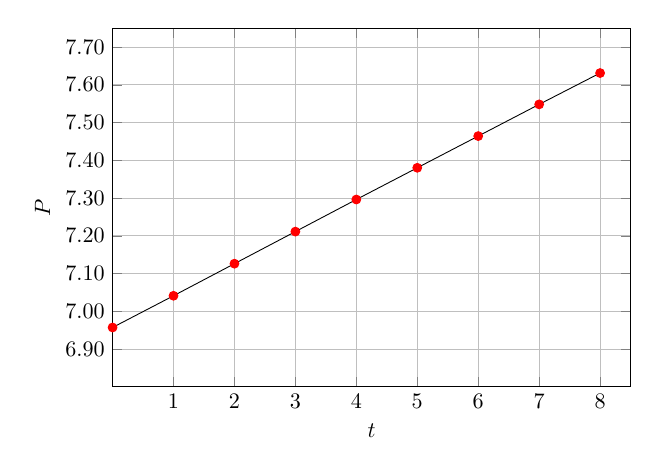
\begin{tikzpicture}[scale=0.8]
\pgfplotstableread{
x y
0 6.957
1 7.041
2 7.126
3 7.211
4 7.296
5 7.380
6 7.464
7 7.548
8 7.631
} \datatable
\begin{axis}[grid=both,
xmin=0,xmax=8.5,
ymin=6.8,ymax=7.75,
xtick={1,2,3,4,5,6,7,8},
ytick={6.9,7.0,...,7.7},
yticklabels = {6.90,7.00,7.10,7.20,7.30,7.40,7.50,7.60,7.70},
minor tick={},
xlabel=\(t\), ylabel=\(P\),
x post scale = 1.2
]
% blue lines
\addplot[mark=none] table [x=x, y=y] {\datatable};
% Red dots
\addplot[only marks,red,mark=*] table [x=x, y=y] {\datatable};
\end{axis}
\end{tikzpicture}
\end{center}
\end{solution}


%------------------------------------


\begin{exercise}\label{exercise-1_3-dragon}
The amount of power a dragon must output to carry a knight depends on how fast it is flying, as shown in the table below.
\begin{center}
\begin{tabular}{|c|c|c|c|c|c|}
\hline speed $x$ (mph) & 60 & 70 & 80 & 90 & 100
\\\hline power $y$ (kW) & 23 & 25 & 30 & 36 &45
\\\hline
\end{tabular}
\end{center}

\begin{parts}
    \item Is the amount of power required for the dragon to carry the knight increasing or decreasing as its speed increases? Explain how you arrive at your conclusion from the data in the table.
    \item Is the amount of power required for the dragon to carry the knight changing faster and faster or slower and slower as its speed increases? Explain how you arrive at your conclusion from the data in the table.
\end{parts}
\end{exercise}


\begin{solution}
    \begin{parts}
        \item The amount of power required for the dragon to carry the knight is increasing as the dragon's speed increases. This is evident from the table since the values associated with the power required increase as the speed increases.
        \item The amount of power required for the dragon to carry the knight is increasing faster and faster as the dragon's speed increases. This is evident from the table since each time the speed increases by 10 miles per hour starting at 60 miles per hour, the power required to carry the knight increases by more and more.
    \end{parts}
\end{solution}


%------------------------------------


\begin{exercise}
Sketch the graph of the function given numerically in Exercise~\ref{exercise-1_3-dragon} and use it to answer the following questions.


\begin{parts}
    \item Is the amount of power required for the dragon to carry the knight increasing or decreasing as its speed increases? Explain how you arrive at your conclusion from the graph.
    \item Is the amount of power required for the dragon to carry the knight changing faster and faster or slower and slower as its speed increases? Explain how you arrive at your conclusion from the graph.
\end{parts}

\end{exercise}



\begin{solution}

\begin{center}
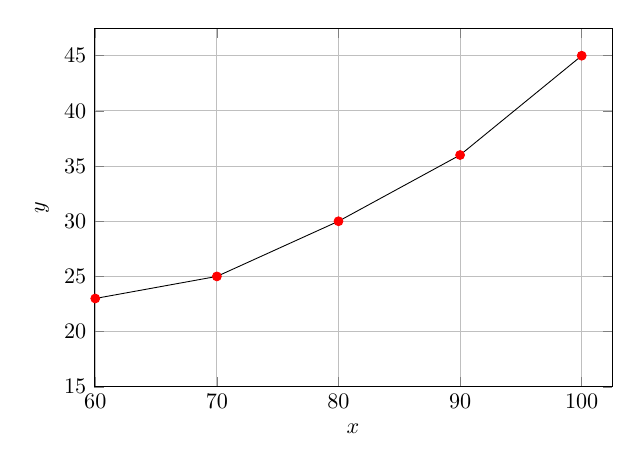
\begin{tikzpicture}[scale=0.8]
\pgfplotstableread{
x y
60 23
70 25
80 30
90 36
100 45
} \datatable
\begin{axis}[grid=both,
xmin=59.9,xmax=102.5,
ymin=15,ymax=47.5,
xtick={60,70,80,90,100},
xticklabels = {60,70,80,90,100},
ytick={15,20,25,30,35,40,45,50},
yticklabels = {15,20,25,30,35,40,45,50},
minor tick={},
xlabel=\(x\), ylabel=\(y\),
x post scale = 1.2
]
% blue lines
\addplot[mark=none] table [x=x, y=y] {\datatable};
% Red dots
\addplot[only marks,red,mark=*] table [x=x, y=y] {\datatable};
\end{axis}
\end{tikzpicture}
\end{center}

\begin{parts}
        \item The amount of power required for the dragon to carry the knight is increasing as the dragon's speed increases. This is evident from the graph since it climbs over the interval $60\leq x \leq 100$.
        \item The amount of power required for the dragon to carry the knight is increasing faster and faster as the dragon's speed increases. This is evident from the graph since each time the speed increases by 10 miles per hour starting at 60 miles per hour, the graph climbs more and more quickly.
\end{parts}
\end{solution}
